\documentclass[border=5pt]{standalone}
\usepackage{amsmath,amssymb}
\usepackage{tikz}
\begin{document}
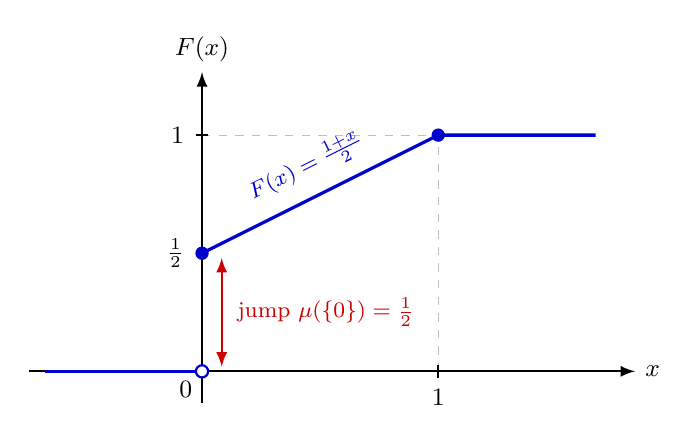
\begin{tikzpicture}[>=latex, font=\small]
  % Axes
  \draw[->, thick] (-2.2, 0) -- (5.5, 0) node[right] {$x$};
  \draw[->, thick] (0, -0.4) -- (0, 3.8) node[above] {$F(x)$};

  % Horizontal reference lines & y-ticks
  \draw[dashed, gray!50] (0, 3.0) -- (5.0, 3.0);
  \draw[dashed, gray!50] (3.0, 0) -- (3.0, 3.0);
  \draw[thick] (-0.08, 1.5) -- (0.08, 1.5);
  \node[left=3pt] at (0, 1.5) {$\tfrac{1}{2}$};
  \draw[thick] (-0.08, 3.0) -- (0.08, 3.0);
  \node[left=3pt] at (0, 3.0) {$1$};

  % x-ticks
  \node[below left] at (0, 0) {$0$};
  \draw[thick] (3.0, -0.08) -- (3.0, 0.08);
  \node[below=3pt] at (3.0, 0) {$1$};

  % F(x) = 0 for x < 0
  \draw[very thick, blue!80!black] (-2.0, 0) -- (0, 0);
  \draw[blue!80!black, thick, fill=white] (0, 0) circle (2.2pt);

  % Jump at x = 0 to (0, 1/2), ramp to (1, 1), flat for x >= 1
  \draw[very thick, blue!80!black] (0, 1.5) -- node[midway, sloped, above=2pt, font=\footnotesize] {$F(x) = \tfrac{1+x}{2}$} (3.0, 3.0) -- (5.0, 3.0);
  \draw[blue!80!black, fill=blue!80!black] (0, 1.5) circle (2.2pt);
  \draw[blue!80!black, fill=blue!80!black] (3.0, 3.0) circle (2.2pt);

  % Annotations
  \draw[<->, thick, red!80!black] (0.25, 0.06) -- node[right=2pt, font=\footnotesize] {jump $\mu(\{0\}) = \tfrac{1}{2}$} (0.25, 1.44);
\end{tikzpicture}
\end{document}
